\documentclass{report}

\input{preamble}
%%%%%%%%%%%%%%%%%%%%%%%%%%%%%%%%%%%%%%%%%%%%%%%%%%%%%%%%%%%%%
% Custom title section
\newcommand{\classinfo}[3]{
    \begin{center}
        {\Large \textbf{#1}} \\ % Class name
        \vspace{0.5cm}
        {\Large #2} \\ % Lecture topic
        \vspace{0.5cm}
        {\large #3}   % Date
    \end{center}
    \vspace{0.5cm} % Add spacing below the title
}
%%%%%%%%%%%%%%%%%%%%%%%%%%%%%%%%%%%%%%%%%%%%%%%%%%%%%%%%%%%%%
% Define custom theorem command with optional numbering and inline separator
\newcommand{\thm}[3][]{ % [#1] is optional, #2 is title, #3 is content
    \noindent\textbf{#2} % Title in bold
    \ifx&#1& % Check if optional input is empty
        % No optional input, skip number
    \else
        \ \textbf{#1} % Include the optional number, bold with space
    \fi
    \ --- % Add the separator
    #3 % Theorem content
}
%%%%%%%%%%%%%%%%%%%%%%%%%%%%%%%%%%%%%%%%%%%%%%%%%%%%%%%%%%%%%
% Define custom claim command with optional numbering and inline separator
\newcommand{\clm}[3][]{ % [#1] is optional, #2 is title, #3 is content
    \noindent\textbf{#2} % Title in bold
    \ifx&#1& % Check if optional input is empty
        % No optional input, skip number
    \else
        \ \textbf{#1} % Include the optional number, bold with space
    \fi
    \ --- % Add the separator
    #3 % claim content
}
%%%%%%%%%%%%%%%%%%%%%%%%%%%%%%%%%%%%%%%%%%%%%%%%%%%%%%%%%%%%%
% Define custom corollary command with optional numbering and inline separator
\newcommand{\crl}[3][]{ % [#1] is optional, #2 is title, #3 is content
    \noindent\textbf{#2} % Title in bold
    \ifx&#1& % Check if optional input is empty
        % No optional input, skip number
    \else
        \ \textbf{#1} % Include the optional number, bold with space
    \fi
    \ --- % Add the separator
    #3 % corollary content
}
%%%%%%%%%%%%%%%%%%%%%%%%%%%%%%%%%%%%%%%%%%%%%%%%%%%%%%%%%%%%%
% Define custom lemma command with optional numbering and inline separator
\newcommand{\lma}[3][]{ % [#1] is optional, #2 is title, #3 is content
    \noindent\textbf{#2} % Title in bold
    \ifx&#1& % Check if optional input is empty
        % No optional input, skip number
    \else
        \ \textbf{#1} % Include the optional number, bold with space
    \fi
    \ --- % Add the separator
    #3 % lemma content
}
%%%%%%%%%%%%%%%%%%%%%%%%%%%%%%%%%%%%%%%%%%%%%%%%%%%%%%%%%%%%%
% Custom proof command
\newcommand{\proof}[2]{ % #1 is the proof content
    \vspace{0.3cm} % Add space before the proof
    \noindent\textit{#1} % "Proof" in italics
    \hspace{0.2cm} #2 % Proof content
    \hfill$\square$ % QED symbol at the end
    \vspace{0.3cm} % Add space after the proof
}
%%%%%%%%%%%%%%%%%%%%%%%%%%%%%%%%%%%%%%%%%%%%%%%%%%%%%%%%%%%%%

\input{letterfonts}

\usepackage{amsmath}
\usepackage{pgf,tikz}
\usetikzlibrary{positioning,shapes,fit,calc}

\title{\Huge{Math 125}\\Course Notes}
\author{\huge{Matteo Costagliola}}
\date{\today}

\begin{document}

\maketitle
\newpage% or \cleardoublepage
% \pdfbookmark[<level>]{<title>}{<dest>}
\pdfbookmark[section]{\contentsname}{toc}
\tableofcontents
\pagebreak
\chapter{Set Theory}
\section{Definitions and The Element Method of Proof}
\subsection{Definitions}
\dfn{}{
Let $S$ denote a set and $a$ an element of set $S$.
$a\in S$ means that $a$ is an element of $S$. $a\notin S$ means that $a$ is not an element of $S$.
If $S$ is a set and $P(x)$ is a property that elements of $S$ may or may not satisfy, then a set $A$ may be defined by writing
\[ A = \{x\in S \mid P(x)\} \]
Read "$A$ is the set of all $x$ in $S$ such that $P(x)$."
}

\dfn{Subsets}{$A\subseteq B \Leftrightarrow \forall x,\text{ if } x\in A \text{ then } x\in B$}
\nt{Since the definition is a universal statement, the negation is existential.\\
\[ A\notin B \Leftrightarrow \exists x \text{ such that } x\in A \text{ and } x\notin B \] }

\dfn{Proper Subsets}{$A\subset B \Leftrightarrow$
\begin{enumerate}
    \item [(1)] \( A\subseteq B \) 
    \item [(2)] \( \exists x \text{ such that }x\in B \text{ and } x\notin A \) 
\end{enumerate}
}
\pagebreak
\ex{}{
    Let $A=\{1\}, B=\{1,\{1\}\}$
    \nt{A set with one element is a \underline{singleton}}
    \begin{enumerate}
        \item [(a)] Is $A\subseteq B$?
        \item [(b)] Is $A\subset B$?
    \end{enumerate}
    \sol{
    \begin{enumerate}
        \item [(a)] Yes, $\forall x$, if $x\in A$ then $x\in B$
        \item [(b)] Yes, $\exists x$ such that $x\in B$ and $x\notin A$
    \end{enumerate}
    }
}
\subsection{Element Method of Proof}
\dfn{Element Method of Proof}{
    Let sets $X$ and $Y$ be given. To prove that $X\subseteq Y$,
    \begin{enumerate}
        \item [(1)] Suppose that $x$ is a particular but arbitrarily chosen element of $X$
        \item [(2)] Show that $x$ is and element of $Y$
    \end{enumerate}
}
\ex{}{
    Define sets $A$ and $B$ as follows:
    \[ A=\{m\in \mathbb{Z}\mid m=6r+12 \text{ for some } r\in \mathbb{Z}\} \]
    \[ B=\{n\in \mathbb{Z}\mid n=3s \text{ for some } s\in \mathbb{Z} \} \]

    \begin{enumerate}
        \item [(a)] Prove that $A\subseteq B$
        \item [(b)] Disprove that $B\subseteq A$
    \end{enumerate}

    \begin{myproof}Show that $A\subseteq B$\\
        Let $x\in A$ (We must show that $x\in B$, by definition of $B$ we must show that $x=3\cdot$ some integer)
        By definition of $A$, there is an integer $r$, such that $x=6r+12$.
        Let $s=2r+4$, then $s\in \mathbb{Z}$ as products and sums of integers are integers, and so $3s\in B$ by definition of $B$.
        Also, $3s=3(2r+4)=6r+12=x$, thus by definition of $B$, $x$ is an element of $B$.

    \end{myproof}

    \begin{myproof}Show that $B\nsubseteq A$\\
        Let $x\in B$, $x=3s$ by definition of $B$. Let $x=3=3\cdot 1$, and set this equal to the definition of $A$.
        $6r+12=3$
        \begin{align*}
         6r+12 &= 3 \text{ by assumption} \\
         2r+4 &= 1 \text{ by diving both sides by 3 } \\
         2r &= -3 \text{ by subtracting 4 from both sides } \\
         r &= \frac{-3}{2} \text{ by dividing both sides by 2 } \\
        \end{align*}

    \end{myproof}
}
\subsection{Set Equality}
\dfn{Set Equality}{
    Given sets $A$ and $B$, $A=B\Leftrightarrow A\subseteq B$ and $B\subseteq A$.
}
\ex{}{
    Define sets $A$ and $B$ as follows:
    \[ A=\{m\in \mathbb{Z}\mid m=2a \text{ for some integer a}\} \]
    \[ B=\{n\in \mathbb{Z}\mid 2b-2 \text{ for some integer b}\} \]
    Show that $A=B$
    \begin{enumerate}
        \item [(a)] \begin{myproof}
            $A\subseteq B$
            Let $x\in A$, by the definition of $A$ there exists an integer $a$ such that $x=2a$.
            Let $b=a+1$, then $b\in \mathbb{Z}$ as it is a sum of integers.
            Also $2b-2=2(a+1)-2=2a+2-2=2a=x$.
            Thus by definition of $B$, $x\in B$.
            Hence $A\subseteq B$.
        \end{myproof}
        \item [(b)] \begin{myproof}
            Let $x\in B$, by the definition of $B$ there exists an integer $b$ such that $x=2b-2$.
            Let $a=b-1$, then $a\in \mathbb{Z}$ as it is a difference of integers.
            Also $2a=2(b-1)=2b-2=x$
            Thus by the definition of $A$, $x\in A$.
            Hence $B\subseteq A$. 
        \end{myproof}
    \end{enumerate}
    Thus we have shown that $A=B$.
}
\subsection{Operations On Sets}
\dfn{Set Operations}{
    Let $A$ and $B$ be subsets of a universal set $U$.
    \begin{itemize}
        \item The \underline{union} of $A$ and $B$, denoted $A\cup B$, is the set of all elements in either $A$ or $B$.
        \item The \underline{intersection} of $A$ and $B$, denoted $A\cap B$, is the set of all elements common to both $A$ and $B$.
        \item The \underline{difference} of $B$ minus $A$, denoted $B-A$, is the set of all elements in $B$ not in $A$.
        \item The \underline{complement} of $A$, denoted $A^\mathsf{c}$, is the set off all elements of $U$ that are not in $A$.
        \\
        Symbolically,
        \begin{align*}    
        A\cup B &= \{x\in U\mid x\in A \text{ or }x\in B\} \\
        A\cap B &= \{x\in U\mid x\in A \text{ and }x\in B\} \\
        B-A &= \{x\in U\mid x\in B \text{ and }x\notin A\} \\
        A^\mathsf{c} &= \{x\in U\mid x\notin A\}
        \end{align*}
    \end{itemize}
}
\dfn{Repeated Operations On Sets}{
    Given sets $A_{0},A_{1},A_{2},...$ that are subsets of a universal set $U$ and given a nonnegative integer $n$,
    \begin{align*}
    \bigcup_{i=0}^{n}A_{i} &= \{x\in U\mid x\in A_{i} \text{ for at least one }i=1,2,...,n\} \\
    \bigcup_{i=0}^{\infty}A_{i} &= \{x\in U\mid x\in A_{i} \text{ for at least one positive integer }n\} \\
    \bigcap_{i=0}^{n}A_{i} &= \{x\in U\mid x\in A_{i} \text{ for every }i=1,2,...,n\} \\
    \bigcap_{i=0}^{\infty}A_{i} &= \{x\in U\mid x\in A_{i} \text{ for every positive integer }i\} 
    \end{align*}
    }
\subsection{The Empty Set}
\dfn{The Empty Set}{
    The empty set, denoted $\emptyset$, is a set containing no elements.
    \[ \emptyset = \{\} \]
}
\subsection{Partitions of Sets}
\dfn{Disjoint Sets}{
    Two sets are called \underline{disjoint} if, and only if, they have no elements in common.
    \[ A\text{ and }B \text{ are disjoint }\Leftrightarrow A\cap B=\emptyset \]
}
\ex{}{
    Let $A=\{1,3,5\}$ and $B=\{2,4,6\}$. Are $A$ and $B$ disjoint?\\
    \sol{\\
        \indent $A\cap B=\{\}=\emptyset$, yes $A$ and $B$ are disjoint.
    }
}
\dfn{Mutually Disjoint Sets}{
    Sets $A_{1},A_{2},A_{3},...$ are \underline{mutually disjoint} (or pairwise disjoint or nonoverlapping) if, and only if, no two sets $A_{i}$ and $A_{j}$ with distinct subscripts have any elements in common.
    More precisely, for all integers $i$ and $j=1,2,3,...$
    \[ A_{i}\cap A_{j} = \emptyset \text{ whenever }i\neq j \]
}
\ex{}{
    Let $A_{1}=\{3,5\},A_{2}=\{1,4,6\},\text{ and }A_{3}=\{2\}$.
    Are $A_{1},A_{2},\text{ and }A_{3}$ mutually disjoint?
    \\
    \sol{\\
        \indent Yes they are disjoint as $A_{1}\cap A_{2}\cap A_{3}=\emptyset$.
    }
}
\dfn{Partitions}{
    A finite or infinite collection of nonempty sets $\{A_{1},A_{2},A_{3},...\}$ is a partition of a set $A$ if, and only if,
    \begin{enumerate}
        \item [(1)] $A$ is the union of all the $A_{i}$.
        \item [(2)] The sets $A_{1},A_{2},A_{3},...$ are mutually disjoint.
    \end{enumerate}
    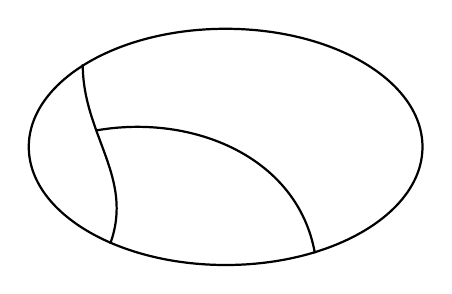
\begin{tikzpicture}
        \node[draw,ellipse,minimum width=5cm,minimum height=3cm,thick](ell)at(0,0){};

        \draw[black,thick] (ell.150) to [out=-90,in=70] coordinate[pos=0.35](p1)(ell.220);
        \draw[black,thick] (p1) to [out=10,in=100] (ell.310) coordinate[pos=0.55](p2);
    \end{tikzpicture}
}
\subsection{Power Sets}
\dfn{Power Set}{
    Given a set $A$, the power set of $A$, denoted $\mathcal{P}(A)$, is the set of all subsets of $A$.
    \nt{The power set of $A$ with length $n$, has length $2^{n}$.}
}
\ex{}{
    Let $A=\{x,y\}$, find $\mathcal{P}(A)$.\\
    \sol{\\
    \indent $\mathcal{P}(A)=\{\emptyset,\{x\},\{y\},\{x,y\}\}$
    }
}


\end{document}
